
\documentclass[a4paper,10pt]{article}
%\usepackage{fullpage}
\usepackage[swedish]{babel}
\usepackage{todonotes}

\usepackage{url}
\usepackage{titlesec}

%\usepackage{algorithmicx}
\usepackage{algorithm}
\usepackage{algpseudocode}
\algnewcommand{\LineComment}[1]{\State \(\triangleright\) #1}
\algnewcommand{\Continue}{\textbf{continue}}
\algnewcommand{\Vspace}{\item[]}
\algnewcommand{\To}{\textbf{to}~}

\usepackage{mathtools}
\DeclarePairedDelimiter\ceil{\lceil}{\rceil}
\DeclarePairedDelimiter\floor{\lfloor}{\rfloor}
\newcommand{\addeq}{\mathrel{+}=}
\newcommand{\subeq}{\mathrel{-}=}
\newcommand{\unioneq}{\mathrel{\cup}=}
\newcommand{\addadd}{\mathrel{++}}
\newcommand{\subsub}{\mathrel{--}}

\usepackage{framed}

%\usepackage[section]{placeins}

\usepackage{graphicx}
\usepackage{caption}
\usepackage{subcaption}

\usepackage{amsmath}

\title{1TE717 Digitalteknik och Elektronik \\ \textbf{Digital överföring av ljudvågor över RF-radio}}

\author{Bj{\"o}rn Forsberg \and Sven Lundgren \and Jonathan Sharyari}
%\textwidth 5.5in 
%\oddsidemargin 0.5in 

\begin{document}

\maketitle

\begin{abstract}

Denna rapport beskriver en implementation av ett system för digital 
överföring av ljud som en del av det projekt som ingår i kursen Digitalteknik 
och Elektronik (1TE717). Systemet använder en mikrofon för att fånga upp 
ljudvågor, vilka sedan konverteras till en digital signal och sänds via radio 
till en mottagare. Mottagaren konverterar tillbaka signalen till en analog 
representation som sedan kan spelas upp på en högtalare. Den digitala 
överföringen minskar risken för störningar, då risken att en etta och nolla ska 
flippa är mindre än risken för störningar på en analog signal.

Vid enklare tester visar sig systemet kapabelt att föra över mycket exakta 
signaler från sändare till mottagare. Det är dock mycket känsligt för att hamna
i otakt, i det att överföringen inte har någon tydlig början och slut. I och med
detta måste mottagaren manuellt synkronisera signalen. Detta måste dock endast
göras en gång vid systemstart. Slutligen använder denna implementation en delad
klocksignal mellan sändare och mottagare, vilket reducerar den praktiska 
användbarheten av systemet. Det lämnas till framtida arbete att implementera en
distribuerad klockning av systemet.
\end{abstract}

\section{Inledning}

Att överföra ljud elektroniskt mellan två punkter är ett av de största 
genombrotten inom kommunikation. Det har tillåtit vänner och familjer  att hålla 
kontakten över stora avstånd, gjort det möjligt för stater att kommunicera i 
realtid.

Traditionellt sett har ljudsignalerna överförts från vibrationer i luften till
förändringar i elektrisk spänning med hjälp av en mikrofon. I denna analoga 
representation, motsvaras tryckförändringar i luften direkt av 
spänningsförändringar i mikrofonens utsignal. På motsvarande sätt överförs de
elektriska signalerna tillbaka till ljudsignaler via en högtalare, genom att 
framkalla tryckförändringar i luften motsvarande spänningsförändringarna i
den elektriska signalen.

I dag sker allt större delar av världens informationsöverföring i digital form, 
där informationen istället uttrycks i sekvenser av höga (t.ex. $5V$) och låga
(t.ex. $0V$) signaler. För att representera ljudvågor digitalt behöver således 
tryckförändringarna i luften översättas till diskreta värden, som kan 
representeras av ett tal.
Exempelvis kan intervallet $[u^{min}, u^{max}]$ delas upp i $n$ diskreta 
delintervall, var och en representerad av ett binärt tal. Ju högre man väljer
$n$, desto fler bitar behövs för att representera alla delintervall. Antalet 
intervall som kan representeras ges av uttrycket $n = 2^b$ där $b$ är antalet 
bitar som används för att uttrycka värdet. Elektriska komponenter som översätter
analoga spänningar till dess digitala representation kallas 
analog-till-digital-omvandlare (AD-omvandlare, ADC). 
För att återföra den digitala signalen till sin analoga form används en
digital-till-analog-omvandlare (DA-omvandlare, DAC), vars funktion är
inversen av ADC:ns. En komplett lista på komponenter som använts i projektet
presenteras i tabell \ref{tab:komponenter}.

Denna rapport presenterar ett projekt om $4 hp$, i vilket ett 
ljudöverföringssystem presenteras. Med hjälp av en mikrofon fångas en 
ljudsignal upp, omvandlas till en digital representation, varpå denna digitala 
representation överförs seriellt via radiovågor till en mottagare. Mottagaren 
omvandlar i sin tur den digitala representationen tillbaka till en analog signal 
som kan omvandlas till ljud av en högtalare.

Att gå igenom dessa steg för att omvandla en analog signal till en digital, för
att sedan direkt återföra den till den analoga representationen kan låta 
onödigt, men motiveras utav den lägre störningsrisken i digital överföring. 
Detta eftersom att en störning på en analog signal överlagras in i signalen, och
det är kostsamt att rensa ut dessa störningar. I motsats kommer en störning på
en digital signal i normalfallet inte påverka informationen i signalen, eftersom
att störningen måste vara mycket stor för att signalens betydelse ska skifta
mellan logiskt hög till låg eller vice versa.


\section{Genomförande}

Implementeringen av kretsen gjordes med ett enkelt kombinatoriskt nät som ger
styrsignalerna till ADC och DAC. Ut- respektive insignalerna till ADC och DAC
förs sedan över via radio. De komponenter som använts presenteras i Tabell 
\ref{tab:komponenter}. Resterande del av denna sektion är uppdelat i fyra
undersektioner, den första beskriver implementationen av mikrofonkretsen, 
varefter den andra beskriver implementationen av sändaren, och slutligen den 
tredje beskriver implementationen av mottagaren. För att spela upp
utsignalen användes en färdig högtalare inbyggd i kopplingsborden som användes,
och därför beskrivs denna komponent ej närmre. Slutligen beskrivs hur de 
synkrona komponenterna i systemet klockas.

\begin{table}
    \centering
    \begin{tabular}{|l|l|}
    \hline
    1 st & Texas Instruments ADS7816P, 12-bit serial ADC \\
    1 st & Texas Instruments DAC7611P, 12-bit serial DAC \\
    1 st & Seriell radiosändare och mottagare \\
    1 st & Mikrofon \\
    2 st & 4-bitars räknare \\
    1 st & 4-vägs AND-grind\\
    1 st & 2-vägs AND-grind \\
    1 st & 2-vägs XOR-grind \\
    1 st & NOT-grind \\
	 & Funktionsgenerator \\
    \hline
    \end{tabular}
    
    \caption{Komponenterna som använts för att implementera systemet.}
    \label{tab:komponenter}

\end{table}

\subsection{Mikrofon}
I det här projektet användes mikrofonen \todo{???}. I databladet för mikrofonen 
hittas den grundläggande krets som krävs för att omvandla ljud till en analog 
elektrisk signal, se figure \ref{mikrofon} 
\todo{Bilden finns i databladet, men jag vetefan}. 
Denna krets skapar en ytterst låg signal, uppemot 10 millivolt. För att på ett 
bra sätt kunna digitalisera signalen användes dels en operationsförstärkare för 
att förstärka signalen, dels en operationsförstärkare för att lyfta signalen så 
att signalen skulle röra sig inom det intervall som AD-omvandlaren är designad 
för, 0 till 5 Volt.



\subsection{Sändare}

Den mest centrala komponenten i sändaren är ADC:n, som konverterar den analoga
signalen från mikrofonen till en 12-bitars digital signal som sedan sänds över
radio.

Det finns ett mycket stort utbud av integrerade kretsar för ADC:er på marknaden,
med flera inbördes olika egenskaper. Det första att ta hänsyn till vid valet av
ADC är seriell eller parallel utsignal. Eftersom att utsignalen skickas över 
radio som en seriell signal är valet av seriell ADC uppenbart. För seriella 
komponenter finns sedan åtskilliga val vad gäller protokoll som kontrollerar när
och hur data skickas ut från komponenten. I detta fall föll valet på en 
SPI-bestyckad ADC, eftersom att SPI är ett förhållandevis enkelt protokoll, och
därmed lätt att kontrollera med hjälp av enkla kombinatoriska nät, i motsats 
till mer avancerade protokoll där en mikrokontroller är mer eller mindre
nödvändig. Eftersom att SPI definerar hur data förs över rent fysiskt mycket
hårdare än det definerar vilken data som skickas, finns det flera olika 
implementationer av dataprotokollet.

Det slutgiltiga valet föll på $ADS7816P$ \cite{adc}, en SPI-bestyckad 12-bitars 
ADC med ett mycket enkelt dataprotokoll, se Figur \ref{fig:adcproto}, vilken 
därför kräver ett mycket enkelt kombinatoriskt när för att styra. ADC:n använder 
fyra klockcykler för att sampla en inkommande signal, och 12 cycler för att
seriellt sända ut dess digitala representation. Sampling påbörjas då 
styrsignalen \emph{CS} (Chip Select) går från hög till låg. Detta resulterar i 
sanningstabellen i tabell \ref{tab:adc} och det motsvarande kombinatoriska nätet 
i Figur \ref{fig:adccircuit}.

\begin{figure}
\centering
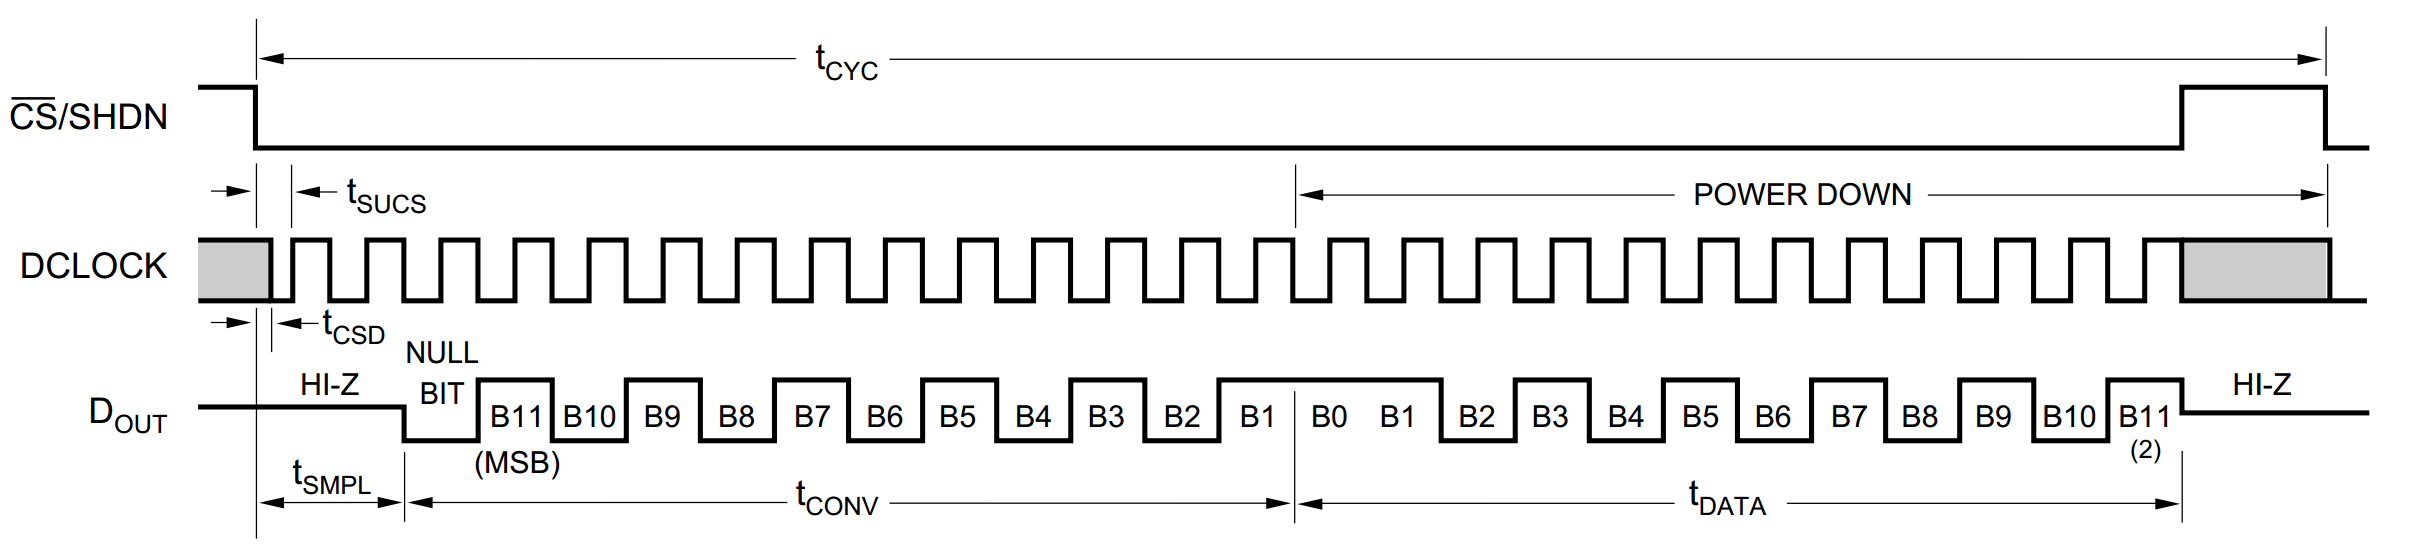
\includegraphics[width=\textwidth]{adcdiagram.png}
\caption{Dataprotokoll för AD-omvandlaren.}
\label{fig:adcproto}
\end{figure}

\begin{table}
\centering
\begin{tabular}{| c c c c || c |}
\hline
$x_3$ & $x_2$ & $x_1$ & $x_0$ & $cs$ \\\hline
0 & 0 & 0 & 0 & 0 \\
0 & 0 & 0 & 1 & 0 \\
0 & 0 & 1 & 0 & 0 \\
0 & 0 & 1 & 1 & 0 \\
0 & 1 & 0 & 0 & 0 \\
0 & 1 & 0 & 1 & 0 \\
0 & 1 & 1 & 0 & 0 \\
0 & 1 & 1 & 1 & 0 \\
1 & 0 & 0 & 0 & 0 \\
1 & 0 & 0 & 1 & 0 \\
1 & 0 & 1 & 0 & 0 \\
1 & 0 & 1 & 1 & 0 \\
1 & 1 & 0 & 0 & 0 \\
1 & 1 & 0 & 1 & 0 \\
1 & 1 & 1 & 0 & 0 \\
1 & 1 & 1 & 1 & 1 \\
\hline
\end{tabular}

$cs$ = $x_3 \wedge x_2 \wedge x_1 \wedge x_0$

\caption{Sanningstabell för styrsignaler för AD-omvandlaren.}
\label{tab:adc}
\end{table}

\begin{figure}
\centering
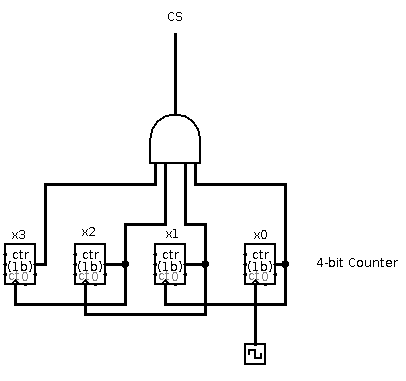
\includegraphics[width=0.8\textwidth]{adccircuit.png}
\caption{Kopplingsschema för styrsignaler för AD-omvandlaren.}
\label{fig:adccircuit}
\end{figure}


\subsection{Mottagare}

Liksom för sändaren är det konverteringen mellan analog och digital data som
är den centrala funktionen i mottagaren. I detta fall är det den digitala 
signalen som mottages över radio som ska konverteras tillbaka till en analog
signal som kan tolkas av högtalaren.

Liksom för valet av ADC i sändaren finns det en stor variation av tillgängliga 
DAC:ar på marknaden. Eftersom att mottagaren ska vara kompatibel med sändaren
är även denna 12-bitars seriell, och liksom ADC:n föll protokollvalet på SPI. 
Även här var en enkel implementation av SPI avgörande och därför valdes 
slutligen $DAC7611P$ \cite{dac} för mottagarens DA-omvandling. 

Denna DAC kräver förutom $CS$-signalen även en $LD$-signal för att ladda in data
i registret, se protokollet i Figur \ref{fig:dacprotocol}. Detta ger ett något 
mer komplicerat grindnät än på sändarsidan, och 3 grindar krävs för att 
producera insignalerna. Grindnätet baseras på sanningstabellen i Tabell 
\ref{tab:dac}, och presenteras i Figur 
\ref{fig:daccircuit}.

\begin{figure}
\centering
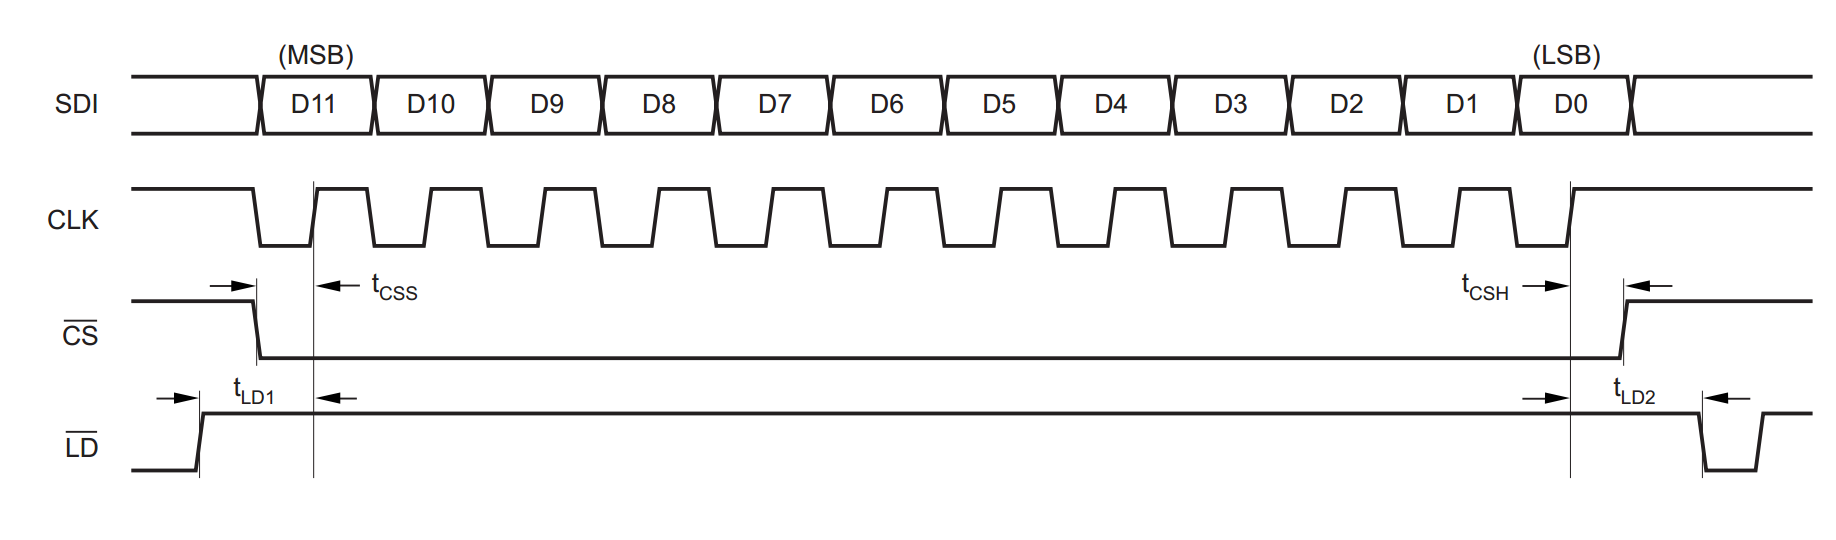
\includegraphics[width=\textwidth]{dacdiagram.png}
\caption{Dataprotokoll för DA-omvandlaren.}
\label{fig:dacprotocol}
\end{figure}

\begin{table}
\centering
\begin{tabular}{|c c c c || c c |}
\hline
$x_3$ & $x_2$ & $x_1$ & $x_0$ & $cs$ & $ld$ \\\hline
0 & 0 & 0 & 0 & 0 & 1 \\
0 & 0 & 0 & 1 & 0 & 1 \\
0 & 0 & 1 & 0 & 0 & 1 \\
0 & 0 & 1 & 1 & 0 & 1 \\
0 & 1 & 0 & 0 & 0 & 1 \\
0 & 1 & 0 & 1 & 0 & 1 \\
0 & 1 & 1 & 0 & 0 & 1 \\
0 & 1 & 1 & 1 & 0 & 1 \\
1 & 0 & 0 & 0 & 0 & 1 \\
1 & 0 & 0 & 1 & 0 & 1 \\
1 & 0 & 1 & 0 & 0 & 1 \\
1 & 0 & 1 & 1 & 0 & 1 \\
1 & 1 & 0 & 0 & 1 & 1 \\
1 & 1 & 0 & 1 & 1 & 0 \\
1 & 1 & 1 & 0 & 1 & 0 \\
1 & 1 & 1 & 1 & 1 & 1 \\
\hline
\end{tabular}

$cs$ = $x_3 \wedge x_2$

$ld$ = $x3 \wedge x_2 \wedge (x_1 \oplus x_0)$

\caption{Sanningstabell för styrsignaler för DA-omvandlaren.}
\label{tab:dac}
\end{table}

\begin{figure}
\centering
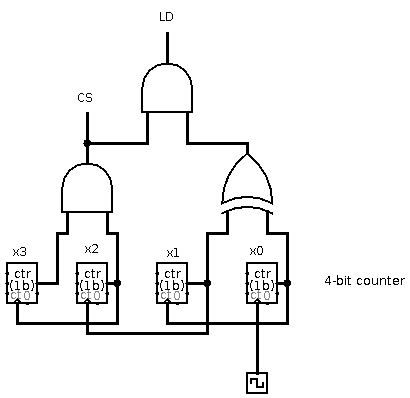
\includegraphics[width=0.8\textwidth]{daccircuit.png}
\caption{Kopplingsschema för styrsignaler för DA-omvandlaren.}
\label{fig:daccircuit}
\end{figure}



\subsection{Trådlös Överföring}
För att seriellt överföra digital information trådlöst användes en sändare och 
en mottagare \todo{Referera till Kjell och Company eller?}. Inga datablad fanns 
tillgängliga för komponenterna, men i praktiken var användandet av dessa 
komponenter var ytterst enkelt. Data som skickas in till mottagaren ut på igen i 
samma format. De kan därför liknas vid en trådlös kabel.

\subsection{Klocka och klockpulser}

Systemet använder sig av flera synkrona integrerade kretsar som kräver en
klockpuls. Klockpulsen styr kretsarnas arbetstakt, och således betyder en hög 
klockpuls att systemet arbetar i en högre takt. Klockpulsen är i detta system 
input till de två integrerade kretsar som agerar sändare och mottagare, där den 
styr hastigheten på kretsernas räknarkomponent. I figur \ref{fig:adccircuit} och 
\ref{fig:daccircuit} kan observeras att var sextonde klockpuls ger så kallad 
\textit{chip select} signal i båda kretsarna, vilket innebär att AD- eller 
DA-omvandlaren ska börja sampla ett nytt värde. Detta i sin tur innebär att 
systemets verkliga arbetstakt gällande konvertering mellan analoga och digitala 
ljudsignaler är $\frac{1}{16}$ av den givna klockfrekvensen.

Konverteringi av tidskontinuerliga signaler till tidsdiskreta signaler beskrivs 
av \textit{Nyquist-Shannons samplingsteorem} \cite{sampling}. Teoremet säger i 
grova drag att för att undvika fel vid diskret sampling av tidskontinuerliga 
signaler bör samplingstakten vara minst dubbla signalens bandbredd. I detta 
projekt antas en bandbredd på $4KHz$ täcka det frekvensband som krävs för att 
fånga upp alla nyanser av mänskligt tal. Samplingsfrekvensen måste då vara 
minst $8KHz$ vilket i sin tur innebär att systemets klockfrekvens måste vara 
minst $16 \times 8KHz = 128KHz$.

Då en snabb klockpuls måste ges till hela systemet för att garantera tillräcklig 
kvalitet på ljudsignalen krävs att de komponenter som ingår i systemet tål denna 
höga klockpuls. Dessa komponenter inkluderar räknare, ADC och DAC.

Eftersom att klocksynkronisering är ett stort och välkänt problem, har det 
utelämnats i detta projekt, och klockpulsen delas således av sändare och 
mottagare i den nuvarande implementationen. Att skapa en implementation av denna 
krets med synkronisering skulle innebära en relativt hög extra 
arbetsbelastining, och vi har här valt att använda en delad klocka för att 
synkronisera sändare och mottagare. En ungefärlig lösning på problemet beskrivs 
dock i Sektion \ref{synkronisering}.


\section{Resultat}

Det implementerade systemet klarar av att relativt störningsfritt överföra 
ljudsignaler mellan sändaren och mottagaren. Då en gemensam klocka användes 
krävdes ingen synkronisering under körning, men däremot krävs synkronisering 
initialt då komponenterna aktiveras vid olika tidpunkter. För att initialt 
synkronisera sändaren och mottagaren skickades en hög reset-signalen till DAC:en 
med en vanlig tryckknapp. Sannolikheten att komponenterna ska vara i synk efter 
en sådan signal är 1/16, och proceduren upprepades till dess att 
ljudåtergivningen var korrekt. 

I Figur \ref{oscilloskop} kan vi se den ursprungliga analoga ljudsignalen (efter 
förstärkning), jämte den återskapade analoga signalen efter digitalisering. Det 
går enkelt att se hur den återskapade signalen bestårm av ett antal diskreta 
värden.


\begin{figure}
\centering
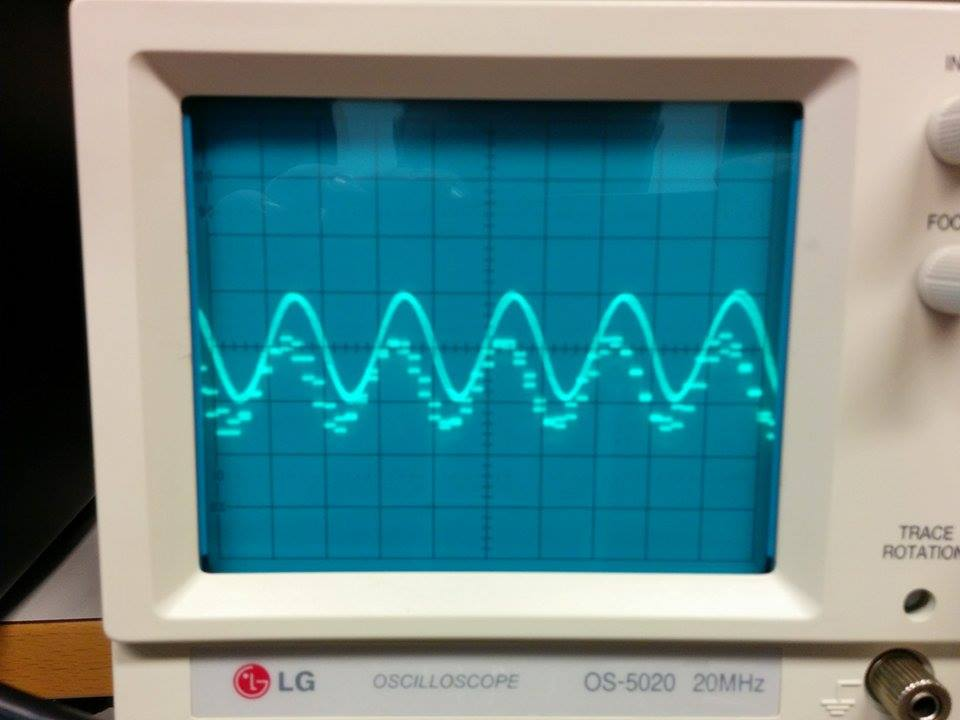
\includegraphics[width=0.8\textwidth]{oscilloskop.jpg}
\caption{Analoga signaler före och efter digitalisering. Den kontinuerliga 
         kurvan utgör den ursprungliga signalen och den streckade kurvan den 
	 återskapade signalen.}
\label{oscilloskop}
\end{figure}


\section{Diskussion}
\subsection{Störningar}
De störningar som uppstår har främst två orsaker. Vid trådlös överföring finns 
alltid risken att data korrumperas eller försvinner, en risk som ökar med 
avståndet mellan sändare och mottagare. Utöver detta så används en samplingstakt 
på 128KHz, med vilken frekvenser upp till 4Khz kan återskapas. Då mänskligt tal 
har frekvenser upp mot 20Khz innebär detta att högre frekvenser än 4Khz 
feltolkas och tillför en mindre störning till signalen. Detta kan lätt åtgärdas 
med ett lågpassfilter som filtrerar bort högre frekvenser.

\subsection{Synkronisering}
\label{synkronisering}
Synkronisering över avstånd är generellt ett svårt problem att lösa, men enklare 
lösningar går att skapa, särskilt i fallet av ljudöverföring eftersom 
feltoleransen är relativt hög. Ett sätt att göra detta är att utnyttja det 
faktum att både ADC och DAC använder 16 klockcykler för att överföra 12 bitar 
data. Under de fyra klockcykler som ADC:n inte skickar data skickas istället 
ettor (höga signaler). Digitalomvandlaren tar då emot fyra ettor innan den 
relevanta informationen, efter den tredje ettan höjs \emph{LD} till hög och vid 
den fjärde sänks \emph{CS} till låg varvid data läses in. Ett sätt att 
synkronisera vore därför att istället för kretsen i figur \ref{dacprotocol}, 
skapa ett nät som läser av den inkommande dataströmmen och höjer \emph{LD} var 
gång den upptäcker tre på varandra följande ettor, och \emph{CS} vid fyra ettor. 
Med en sådan krets skulle information synkroniseras för varje siffra som skickas 
över. Däremot skulle detta innebära att om den binära representationen av den 
siffra som skickas innehåller fyra efter varandra följande ettor skulle detta 
feltolkas, och systemet skulle temporärt vara i osynk.


\section{Bibliografi}

\begin{thebibliography}{hejhej}

\bibitem{sampling}
    {Cand{\`e}s, Emmanuel J and Wakin, Michael B,
    \emph{An introduction to compressive sampling},
    Signal Processing Magazine, IEEE,
    volume 25,
    number 2,
    pages 21-30,
    2008.
}
\end{thebibliography}


\end{document}
